\documentclass[a4paper,11pt]{article}

\usepackage[utf8]{inputenc}

\usepackage{graphicx}
\usepackage{caption}
\usepackage{subcaption}

\usepackage{pgfplots}
\pgfplotsset{compat=1.18} 

\usepackage{minted}

\usepackage{tikz}
\usepackage{pgfplots}

% Required packages
\pgfplotsset{compat=1.18} % Use 1.17+ for groupplots; adjust to your TeX Live
\usepgfplotslibrary{groupplots}

\usepackage[T1]{fontenc}
\usepackage[utf8]{inputenc} % ensure file is UTF-8 to avoid invisible bad chars
\usepackage{lmodern}        % optional but recommended
\usepackage{caption}        % optional

\begin{document}

\title{
    \textbf{A Calculator in C using stack}
}
\author{Mo Wang}
\date{Spring 2026}

\maketitle

\section*{Introduction}

This report delves into the implementation of a calculator in C using reversed Polish notation with a stack. The purpose of the report is to learn practical application of a stack data structure as well as to compare differences between static and dynamic stack, by implementing a simple terminal-based calculator supporting reversed Polish notation.

\section*{Different stack implementations}

Because a stack is an array that supports only push and pop operations, it can be implemented with either with a fixed capacity size or a dynamically growing capacity size. A stack with a fixed capacity size is called a static stack, while the other one that can grow and shrink is called a dynamic stack. Both types of stacks are discussed below.

\subsection*{Static stacks}

A static stack has a fixed maximum capacity or a pre-defined size to fit within the available memory blocks. The stack has a stack pointer (or index) named \texttt{top} that points to the element immediately after the topmost element, effectively pointing to the next free slot, which follows the stack pointer convention. This convention becomes especially clear in an empty stack, where the \texttt{top} index points to the first element at index zero.

\begin{minted}{c}
  typedef struct static_stack{
      unsigned int top;
      unsigned int size;
      int *array;
  } static_stack;
\end{minted}

A static stack has two different operations, push and pop. The push operation overlays the given element above the topmost element of the stack, which means that the element is written using stack index, while incrementing it. On the other hand, pop operation removes the topmost element, revealing the element beneath it, by decrementing the stack index and returning the element at its position. The operations are shown below in functions \texttt{static\_stack\_push} and \texttt{static\_stack\_push}.

\begin{minted}{c}
  void static_stack_push(static_stack *stk, int val) {
      stk->array[stk->top++] = val;
  }

  int static_stack_pop(static_stack *stk) {
      return stk->array[--stk->top];
  }
\end{minted}

However, attempting to push an element beyond its capacity size or pop an element when empty results in accessing out-of-bounds memory and causes undefined behavior. To mitigate this issue, the stack pointer \texttt{top} will be checked before performing any operation. The push operation fails when stack pointer reaches the array capacity (\texttt{stk->top >= stk->size}) while pop operation fails when stack pointer is zero (\texttt{stk->top == 0}).

For reporting operation success, the push function can return \texttt{true} if successful, and the pop function can return a \texttt{Result} struct containing a boolean success flag and an integer value for the popped element. By catching the success flag, the caller function can determine the status of the operation.

\begin{minted}{c}
  typedef struct Result{
      bool success;
      int value;
  } Result;

  bool static_stack_push(static_stack *stk, int val) {...}
  Result static_stack_pop(static_stack *stk) {...}
\end{minted}


\subsection*{Dynamic stacks}

Implementing a dynamic stack (\texttt{dynamic\_stack}) that can grow and shrink is largely similar to implementing a static stack in terms of the \texttt{struct} layout and the creation/destruction routines. The principal difference lies in capacity management: the dynamic stack tracks its current capacity in \texttt{size} and resizes the underlying array by reallocating memory when needed, whereas the static stack’s capacity is fixed at initialization.

During a push operation (\texttt{dynamic\_stack\_push}), if the array is full, the stack allocates a new array with double the previous capacity and copies the existing elements into it before inserting the new item. This geometric growth strategy yields an amortized constant-time complexity of $O(1)$: although an occasional resize costs $O(n)$ due to copying, the cost spread over many subsequent pushes averages to constant time.

\begin{minted}{c}
  bool dynamic_stack_push(dynamic_stack *stk, int val) {
      if (stk->top >= stk->size) {
          unsigned int new_size = stk->size * 2;
          int *new_array = malloc(new_size * sizeof(int));
          if (!new_array){
              return false;
          }
          for (unsigned int i = 0; i < stk->top; i++){
              new_array[i] = stk->array[i];
          }
          free(stk->array);
          stk->array = new_array;
          stk->size = new_size;
      }
      stk->array[stk->top++] = val;
      return true;
  }
\end{minted}

Shrinking the array, on the other hand, is also important to free memory when the number of elements decreases in \texttt{dynamic\_stack\_pop} function equivalence. However, reducing array size whenever it falls below half its capacity can lead to array thrashing during repeatedly growth and shrinks around the same size. To prevent this, the array is only shrunk into half of its capacity when the number of elements drops strictly below one fourth of the current capacity (\texttt{stk->top < stk->size/4}). Additionally, the array will shrink below certain minimum capacity size (\texttt{stk->size > MIN\_STACK\_SIZE}), in this case 4, in order to prevent frequent grow-shrink oscillation of tiny stacks.

\begin{minted}{c}
  Result dynamic_stack_pop(dynamic_stack *stk) {
      if (stk->top == 0) {
          return (Result){ .success = false, .value = 0 };
      }
      
      int popped = stk->array[--stk->top];
      if (stk->top > 0 && stk->top < stk->size/4 && stk->size > MIN_STACK_SIZE){
          unsigned int new_size = stk->size / 2;
          int *new_array = malloc(new_size * sizeof(int));
          if (new_array){
              for (unsigned int i = 0; i < stk->top; i++){
                  new_array[i] = stk->array[i];
              }
              free(stk->array);
              stk->array = new_array;
              stk->size = new_size;
          }
      }
      return (Result){ .success = true, .value = popped };
  }
\end{minted}

\section*{Performance Comparison}

Both stack implementations provide the same functional behavior. The key difference lies in how they handle capacity: a static stack cannot grow beyond its initial size, while a dynamic stack can expand when additional space is required. This flexibility comes at the cost of a slight performance overhead due to occasional memory reallocation.

As illustrated in Figure~1, both stacks exhibit constant-time behavior $O(1)$ for push and pop operations. However, the dynamic stack incurs a small overhead—on the order of a few nanoseconds—compared with the static stack, particularly at input sizes that trigger internal resizing.

\begin{figure}[h]
  \centering
  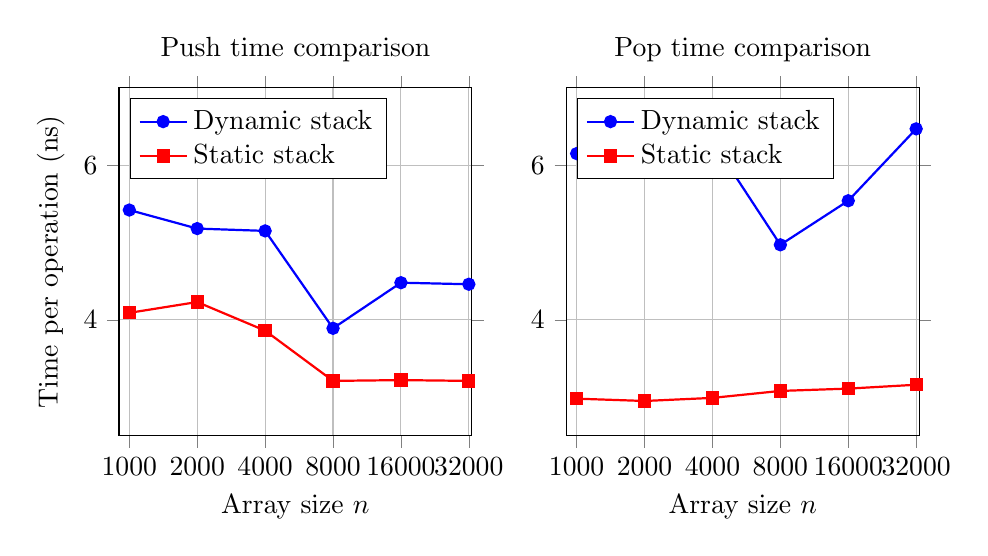
\begin{tikzpicture}
    \begin{groupplot}[
      group style={
        group size=2 by 1,
        horizontal sep=1.2cm
      },
      width=0.5\textwidth,
      height=6cm,
      grid=major,
      tick align=outside,
      xmode=log,
      log basis x={10},
      xmin=900, xmax=33000,
      xtick={1000,2000,4000,8000,16000,32000},
      xticklabels={1000,2000,4000,8000,16000,32000},
      ymin=2.5, ymax=7.0,
      every axis plot/.append style={thick},
      every mark/.append style={mark size=2.5pt}
    ]

      % ---------- (a) Push ----------
      \nextgroupplot[
        title={Push time comparison},
        xlabel={Array size $n$},
        ylabel={Time per operation (ns)},
        legend pos=north west,
        legend cell align={left}
      ]
        % Dynamic push
        \addplot[color=blue, mark=*] coordinates {
          (1000,5.42) (2000,5.18) (4000,5.15) (8000,3.89) (16000,4.48) (32000,4.46)
        };
        \addlegendentry{Dynamic stack}

        % Static push
        \addplot[color=red, mark=square*] coordinates {
          (1000,4.09) (2000,4.23) (4000,3.86) (8000,3.21) (16000,3.22) (32000,3.21)
        };
        \addlegendentry{Static stack}

      % ---------- (b) Pop ----------
      \nextgroupplot[
        title={Pop time comparison},
        xlabel={Array size $n$},
        legend pos=north west,
        legend cell align={left}
      ]
        % Dynamic pop
        \addplot[color=blue, mark=*] coordinates {
          (1000,6.15) (2000,6.29) (4000,6.31) (8000,4.97) (16000,5.54) (32000,6.47)
        };
        \addlegendentry{Dynamic stack}

        % Static pop
        \addplot[color=red, mark=square*] coordinates {
          (1000,2.98) (2000,2.95) (4000,2.99) (8000,3.08) (16000,3.11) (32000,3.16)
        };
        \addlegendentry{Static stack}

    \end{groupplot}
  \end{tikzpicture}
  \caption{Push and pop time comparison between static and dynamic stack implementations (shared axes).}
  \label{fig:stack-push-pop-shared-axes}
\end{figure}

However, the slight performance overhead of using dynamic stack doesn't affect the terminal calculator application, since the program is mostly idle, waiting for keyboard interrupts rather than executing tight loops where tiny performance overhead accumulates. On the other hand, static stacks are unsuitable since it cannot grow arbitrarily large, where the maximum number of operands during processing cannot be determined or estimated beforehand. Based on this, the calculator implements dynamic stack over static stack, since dynamic stack have more suitable benefits in this application.

\section*{Calculator implementation}

With the stack implementations, building a reverse Polish notation terminal calculator becomes straightforward. Each token is passed into the CLI interface delimited by newlines and will be checked for number or operator. If the token is a number, it will be pushed onto the stack, otherwise if it's an operator it's used to pop 2 operands and push the calculated result if the given token is an operator. After processing the current token, the process is repeated over again, until an empty token is passed and the final calculated result will be produced. The structural code can be visualized as below:

\begin{minted}{c}
  #include <string.h>
  
  int main() {
      // allocate a stack resources
      bool running = true;
      while(running) {
          // Read a token from stdin and perform operation
          // running = false when "\n" is read or stack error.
      }
      // Pop the calculated result to stdout
      // deallocate the stack resources
  }
\end{minted}

Terminal user input are read from standard input \texttt{stdin} and written into a char buffer \texttt{buffer} using function \texttt{fgets}. When enter key is pressed, a newline character is fed into standard input and \texttt{fgets} stop reading while storing the user input line including newline and null character to the buffer. 

\begin{minted}{c}
  // Initially allocate a buffer sized 16 bytes
  int n = 16;
  char *buffer = malloc(n);
  fgets(buffer, n, stdin);
  
\end{minted}

Numbers can be distinguished from operators using string compare function \texttt{strcmp} and search string function \texttt{strchr} from \texttt{<string.h>} library. Empty token can be detected by \texttt{strcmp(buffer, "\\n") == 0}, while operators by \texttt{(strchr("+-*/", buffer[0])}.

When a number is detected, it is pushed to the stack. In the meantime, after an operator is detected, two values should be popped out from the stack and calculated as well as pushing the value back to stack. The calculating operation is accomplished by \texttt{apply\_op} that takes the stack and an operator and produce the correct calculation. Operation success or failure is reported by the output boolean flag, \texttt{true} for successed operation, while \texttt{false} for failed operation. The operation can be failed if the stack state is invalid or division by zero attempt is detected.

\begin{minted}{c}
bool apply_op(dynamic_stack *stk, char op) {
    Result b = dynamic_stack_pop(stk);
    Result a = dynamic_stack_pop(stk);
    if (!a.success || !b.success) return false;
    // ...
    if (op == '/' && b.value == 0) return false;
    dynamic_stack_push(stk, ...);
    return true;
}
\end{minted}

The caller function function recieves the status flag of the operation in the application loop and terminate the application program when invalid state error or division by zero attempt occurs. The main application loop is exited while stack resources are deallocated in the process. Using this approach, any invalid user input or invalid program state invariant can be caught and resolved by terminating the program.


\iffalse
Hints:
 - How tokens are read from stdin.
 - How you distinguish numbers from operators.
 - How each operator works (pop two values, compute, push result).
 - How division by zero is handled.
 - How the calculator behaves when the stack is in an invalid state.
\fi



\section*{Testing}
Feeding the reverse Polish notation expression \texttt{4 2 3 * 4 + 4 * + 2 -} into the calculator program produces the result \textbf{42}.

This corresponds to the infix expression which evaluates to the same value. \[ 4 + (2 \cdot 3 + 4) \cdot 4 - 2 \]

\iffalse
Hints:
(MOST IMPORTANT)
This is where you show that you “experimented with both versions of the stack.”
Include:
Example expressions you tested.
Differences in behavior between static and dynamic stacks.
What happens when the static stack overflows.
What happens when you pop from an empty stack.
The evaluation of the example expression:
\fi


\end{document}
